% Created 2022-10-18 ter 18:16
% Intended LaTeX compiler: pdflatex
\documentclass[11pt]{article}
\usepackage[utf8]{inputenc}
\usepackage[T1]{fontenc}
\usepackage{graphicx}
\usepackage{longtable}
\usepackage{wrapfig}
\usepackage{rotating}
\usepackage[normalem]{ulem}
\usepackage{amsmath}
\usepackage{amssymb}
\usepackage{capt-of}
\usepackage{hyperref}
\usepackage{todonotes}
\usepackage[portuges]{babel}
\usepackage{amsthm}
\usepackage[a4paper, total={6in, 8in}]{geometry}
\usepackage{multicol}
\author{Ieremies Vieira da Fonseca Romero}
\date{}
\title{Problema de Dominação Romana}
\hypersetup{
 pdfauthor={Ieremies Vieira da Fonseca Romero},
 pdftitle={Problema de Dominação Romana},
 pdfkeywords={},
 pdfsubject={},
 pdfcreator={Emacs 28.2 (Org mode 9.6)}, 
 pdflang={Portuges}}
\usepackage{biblatex}
\addbibresource{~/arq/bib.bib}
\begin{document}

\maketitle
\begin{abstract}
A Dominação Romana é um problema proposto por \textcite{Stewart1999DefendRomanEmpire} em que desejamos defender o império romano dispondo de um certo número de legiões.
Para isso, cada cidade deve ser protegida de forma que esta possua uma legião ou que uma vizinha dela possua duas legiões.
Assim, deseja-se minimizar a quantidade de legiões distribuídas sem abdicar da segurança do império.

Neste projeto, utilizaremos Programação Linear Inteira (PLI) para modelar o problema.
Objetivamos propor novos modelos de PLI para dominação romana e suas variantes, explorando técnicas como \emph{branch-cut}, \emph{branch-price} e ferramental moderno de PLI.
\end{abstract}

\section{Introdução}
\label{sec:orge94aeb2}
Durante a Segunda Guerra Mundial, General Douglas MacArthur propôs uma estratégia de movimentação que consistia em avançar suas tropas de uma ilha para outra apenas quando ele poderia deixar para trás um número suficiente de tropas (\autocite{Stewart1999DefendRomanEmpire}).
Ele não foi o primeiro a utilizar dessa estratégia: segundo \textcite{Stewart1999DefendRomanEmpire}, referências históricas apontam que o Imperador Constantino, no quarto século A.C., aplicou estratégia similar para defender o Império Romano de invasões dos povos ditos ``bárbaros''.

Para exemplificar o seu uso, considere o mapa do Império Romano simplificado na Figura \ref{fig:mapa}.
Nesse exemplo, o imperador possui \(4\) legiões para serem distribuídas pelo território e ele deseja fazê-lo de forma que todas as cidades sejam consideradas seguras.
Uma região é dita segura, ou coberta, se há uma legião em seu território ou se está conectada a outra região com duas legiões.

\begin{figure}[htbp]
\centering
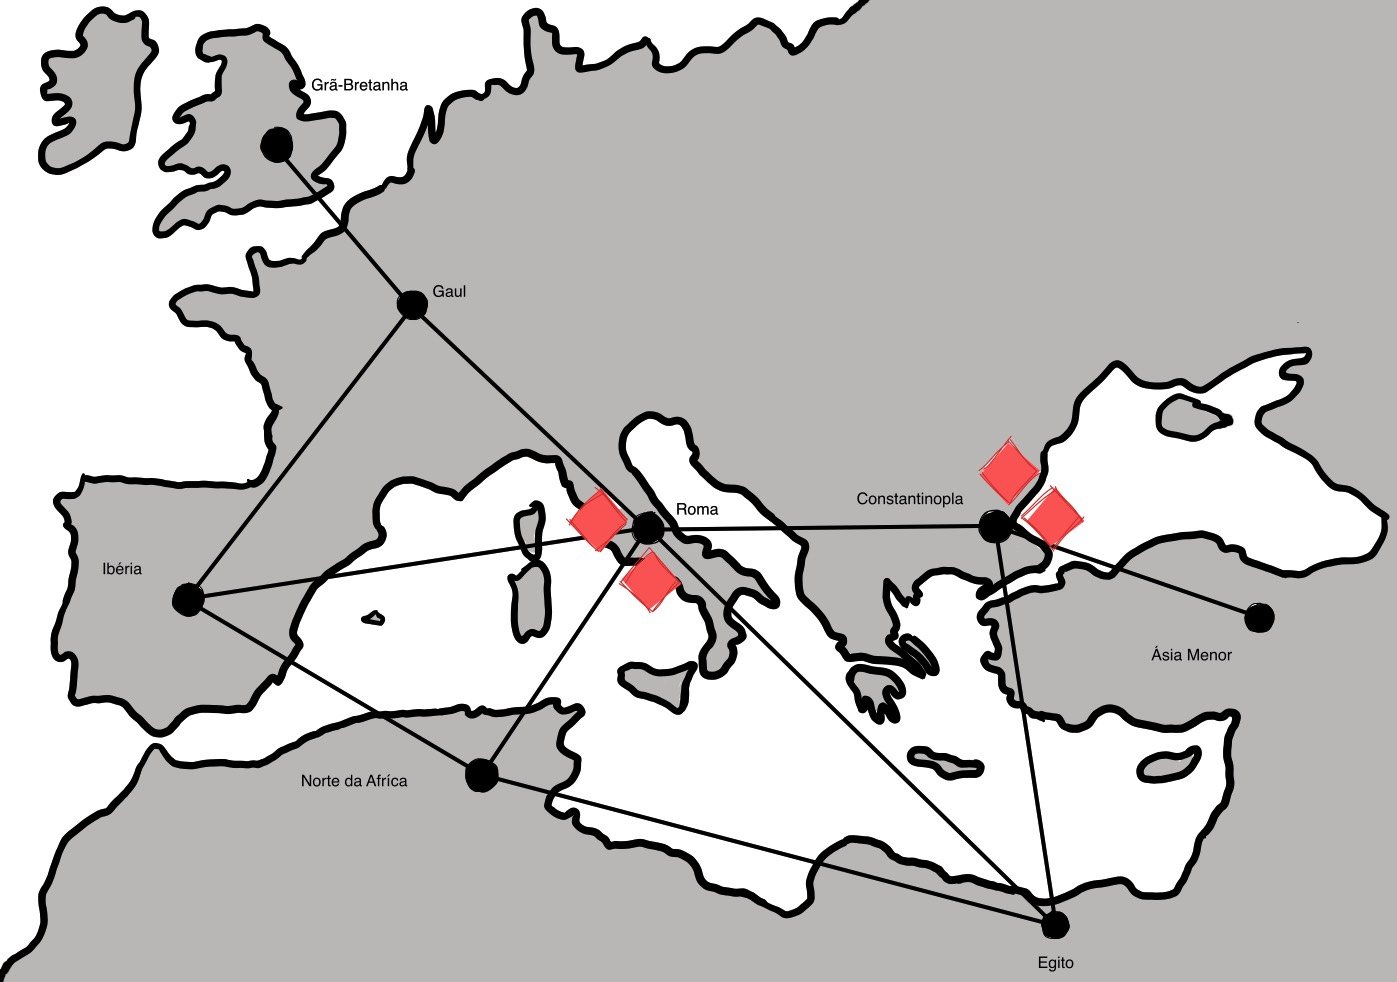
\includegraphics[scale=0.3]{./mapa.jpg}
\caption{\label{fig:mapa}Representação do mapa do Império Romano usada como ilustração do problem, inspirada em \textcite{Stewart1999DefendRomanEmpire}.}
\end{figure}

As aplicações vão além do universo militar: ao alocar estações de serviços de emergência, uma lógica similar à ``segurança'', acima descrita, é muito útil \autocite{GhaffariHadigheh2019Romandominationproblem}.
Além disso, redes sem fio ``ad hoc'', onde um conjunto de usuários com conexões sem fio formam uma rede temporária, sem necessidade de autoridade central ou infraestrutura permanente, constituem outro bom exemplo \autocite{Wu2000Dominationitsapplications}.


\subsection{Modelo matemático}
\label{sec:org4e644aa}
Para um grafo \(G = (V, E)\), dizemos que a \textbf{vizinhança aberta} \(N(v)\) de um vértice \(v\) é definida como o conjunto de vértices adjacentes a \(v\) em \(G\), ou seja, \(N(v) = \{u : (u, v) \in E\}\).
Similarmente, dizemos que a \textbf{vizinhança fechada} \(N[v]\) de um vértice \(v\) é a vizinhança aberta incluindo o próprio \(v\), ou seja, \(N[v] = N(v) \cup \{v\}\).
Para um conjunto de vértices \(s\), a vizinhança aberta desse conjunto é a união das vizinhanças abertas de cada um dos seus vértices (o respectivo pode ser dito para a vizinhança fechada).
Um \textbf{conjunto dominante} de um grafo \(G\) é um subconjunto de vértices \(D\) tal que a vizinhança fechada de \(D\) é o próprio conjunto \(V\).
Por sua vez, o \textbf{número de dominação} de um grafo \(G\), dito \(\gamma(G)\), é a cardinalidade do menor conjunto dominante do grafo \(G\).

O problema de dominação romana é definido em um grafo \(G = (V, E)\) simples, finito e não-direcionado, no qual cada vértice representa uma cidade ou região do império e as arestas são as conexões entre elas \autocite{Cockayne2004Romandominationgraphs}.
Dizemos que uma \textbf{função de dominação romana} é uma função \(f : V \to \{0, 1, 2\}\) na qual \(f(v)\) indica a quantidade de legiões naquela região, de forma que, para qualquer \(v\) tal que \(f(v) = 0\), deve existir \(u\) vizinho a \(v\) cujo \(f(u) = 2\).
Definimos o \textbf{número de dominação romana} de um grafo \(G\) como o menor valor \(f(v), \forall v \in V\), tal que \(f\) é uma função de dominação romana do grafo \(G\).

\subsection{Revisão bibliográfica}
\label{sec:org86e3ee6}
Após a descrição inicial do problema, \textcite{ReVelle2000DefendensImperiumRomanum} apresentaram o desenvolvimento inicial em teoria de grafos.
Além disso, \textcite{Cockayne2004Romandominationgraphs} apresentaram alguns resultados importantes de teoria de grafos sobre o problema, como limitantes e propriedades da função de dominação romana, os quais foram estendidos e aprimorados por \textcite{Xing2006noteRomandomination}, \textcite{Favaron2009Romandominationnumber}, \textcite{Mobaraky2008BoundsRomanDomination}.
Algumas classes especiais de grafos podem ser resolvidas em tempo linear, mas, no caso geral, o problema é NP-difícil (\autocite{Dreyer2000Applicationsvariationsdomination,Klobucar2014SomeresultsRoman,Shang2007RomanDominationProblem}).

\textcite{Ivanovic2016Improvedmixedinteger} utilizaram a meta-heurística \emph{Variable Neightborhood Search} (VNS), obtendo resultados interessantes para as instâncias propostas por \textcite{Curro2014RomanDominationProblem} para o mesmo problema.
Essa meta-heurística parte da ideia de que soluções ótimas são encontradas ``próximas'' de boas soluções. Assim, é possível utilizar busca local e eventuais técnicas de perturbação para escapar de mínimos locais.

Já \textcite{Khandelwal2021RomanDominationGraphs} utilizaram algoritmos genéticos no problema de dominação romana, uma ideia que toma de inspiração da evolução das espécies observadas na natureza.
Partindo de um conjunto de soluções, realizamos ``cruzamentos'' das melhores para produzir novas gerações.
A cada uma, induzimos ``mutações'' aleatórias que alteram certos pontos das soluções, espelhando a realidade e tentando evitar cair em mínimos locais.

\section{Metodologia}
\label{sec:orgbe4b927}
\textbf{Programação Linear} é uma técnica de otimização de problemas a partir da modelagem dos mesmos em \textbf{programas lineares}.
Nestes, definimos uma função objetivo, a qual queremos maximizar ou minimizar com suas variáveis sujeitas a um conjunto de restrições lineares (equações ou inequações lineares) \autocite{Chvatal1983LinearProgramming} . Um programa linear pode ser escrito da seguinte forma:
\begin{alignat*}{4}
& \omit\rlap{minize \quad \quad $\displaystyle cx$} \\
& \mbox{sujeito a}&& \quad & Ax & \geq b  & \quad &  \\
&                 &&       & x               & \in \mathbb{R}_+ &      &
\end{alignat*}

Para encontrar soluções viáveis com valores ótimos, conhecemos o algoritmo \textbf{simplex} que, apesar de ter complexidade exponencial, no caso médio executa em tempo polinomial.

Para alguns problemas, como o de dominação romana, não faz sentido falar em soluções fracionárias, afinal, não conseguimos designar meia legião a uma cidade.
Para isso, restringimos as variáveis aos inteiros, fazendo assim um \textbf{Programa Linear Inteiro}. Caso apenas um subconjunto das variáveis possuam a restrição de integralidade, chamamos esse programa de linear misto.


O que a princípio pode parecer uma pequena alteração, torna o problema computacionalmente ainda mais complexo. Para encontramos boas soluções viáveis para esse tipo de programa, algoritmos como o simplex não são o suficiente. Para isso, utilizamos técnicas como \textbf{branch-and-bound}, que consiste em dividir o problema em subproblemas menores e, durante o processo, encontrar limitantes que permitam diminuir o espaço de busca.

Variações como \textbf{branch-and-cut}, na qual, ao atingir soluções não inteiras na relaxação linear usando o simplex, utilizamos algoritmos de plano de cortes para adicionar mais restrições até a solução fornecida pelo simplex na RL for inteira.
Já para \textbf{branch-and-price}, essa técnica advém da observação que, para grandes problemas, grande parte das variáveis permanecem nulas entre as interações do \emph{branch-and-bound}.
Assim podemos inseri-las conforme progredimos na nossa busca utilizando técnicas de geração de colunas.

\textcite{Ivanovic2016Improvedmixedinteger} propôs duas formulações, como a descrita a baixo, para o problema de dominação romana.
Nesta, para cada vértice \(i\), existem duas variáveis associadas: \(x_i\) real não-negativa e \(y_i\) binária. Se \(x_i < 1\) e \(y_i = 0\), então \(f(i) = 0\); se \(x_i \geq 1\), então \(f(i) = 1\); se \(y_i = 1\), então \(f(i) = 2\).

\begin{alignat*}{4}
& \omit\rlap{minimize  $\displaystyle \sum_{i \in V} x_i+2\sum_{i \in V} y_i$} \\
& \mbox{sujeito a}&& \quad & x_i+y_i+\sum_{j \in N_i} y_j & \geq 1  & \quad & i \in V \\
&                 &&       & x_i               & \in \mathbb{R}_+ &      & i \in V \\
&                 &&       & y_i               & \in \{0,1\}      &      & i \in V
\end{alignat*}

Perceba que soluções onde \(x_i > 1\) e \(y_i = 1\) são viáveis, mas \textcite{Ivanovic2016Improvedmixedinteger} mostra que elas não serão ótimas.

\section{Objetivos}
\label{sec:org2bf008b}
Neste projeto, objetivamos propor novos modelos de PLI para dominação romana e suas variantes explorando técnicas como \textbf{branch-and-cut} e \textbf{branch-and-price}.
Além disso, estudaremos a possibilidade de novos cortes e limitantes para as formulações.

Os algoritmos e modelos propostos serão comparados com as instâncias presentes na literatura, como em \textcite{Curro2014RomanDominationProblem} e, se necessário novas instâncias poderão ser geradas.

Os resultados dos experimentos computacionais serão comparados utilizando técnicas como \textbf{Performance Profile} demonstrado por \textcite{Dolan2002Benchmarkingoptimizationsoftware}.

\printbibliography
\end{document}
